% Light-cone-quantized QCD in 1+1 dimensions, revisited
%
% Structural mirror of Hornbostel, Brodsky & Pauli, PRD 41, 3814 (1990):
% every figure reproduced at much larger K with a full error budget, the
% chiral region reached with the improved Hamiltonian, a tetraquark/hexaquark
% search, and comparison against the 2013-2026 literature.
%
% House rules (enforced by `make check`, see ../docs and the plan):
%  - No numeric literal in prose: every number is a macro from frozen/numbers.tex.
%  - Every caption states N, B, 2K, m/g, LPN, fit window (or "no fit"),
%    and the Hamiltonian.
%  - Improved-Hamiltonian numbers extrapolate in plain 1/K; standard in the
%    Eq. (27) ladder; the two never share a fit.
%  - Section X.E (equal-time cross-check) must be deletable with zero
%    dangling references.
\documentclass[aps,prd,twocolumn,superscriptaddress,nofootinbib]{revtex4-2}

\usepackage{amsmath,amssymb}
\usepackage{graphicx}
\usepackage{xcolor}
\usepackage{hyperref}

\graphicspath{{figs/}}
% frozen v0test — 2026-08-16 — generated file, do not edit
\newcommand{\numAlphaImproved}{1.03}
\newcommand{\numAlphaImprovedDrift}{0.004}
\newcommand{\numAlphaStandard}{1.96}
\newcommand{\numAlphaStandardDrift}{0.008}
\newcommand{\numCapturePctTiny}{0.105}
\newcommand{\numGmorIntercept}{-0.0005 \pm 0.0008}
\newcommand{\numHalvingLogTen}{2444}
\newcommand{\numRatioWorstDevPct}{0.4}
\newcommand{\numTableoneImprovedNBeyondThreeSigma}{0}
\newcommand{\numTableoneImprovedWorstFitonlySigma}{37}
\newcommand{\numTableoneNEntries}{30}
\newcommand{\numTableoneNOutsidePaperTerm}{4}
\newcommand{\numTableoneWorstWeakBarPct}{285}
\newcommand{\numTinyNeightGap}{1513}
\newcommand{\numTinyNeightImprovedMsq}{2.492e-03}
\newcommand{\numTinyNeightStandardMsq}{1.647e-06}
\newcommand{\numTwoBodyExact}{0.779141}
\newcommand{\numTwoBodyImproved}{0.779315}
\newcommand{\numTwoBodyImprovedRel}{2.2e-04}
\newcommand{\numTwoBodyStandard}{0.4536}


\begin{document}

\title{Light-cone-quantized QCD in 1+1 dimensions, revisited}

\author{H.~Lamm}
\affiliation{}

\date{\today}

\begin{abstract}
% Three sentences, mirroring the 1990 abstract's economy: what is
% diagonalized, what is computed, what is new (K reach, error budget,
% chiral region, exotics, modern comparisons).
\end{abstract}

\maketitle

% 01-intro — the 1990→2026 mission statement
\section{Introduction}
\label{sec:intro}

In 1990, Hornbostel, Brodsky and Pauli diagonalized the light-cone
Hamiltonian of SU($N$) gauge theory in one space and one time
dimension~\cite{Hornbostel:1988fb}.  They computed the hadronic spectrum and
wavefunctions across couplings, colors, and baryon number at resolutions
$2K = 16$--$24$, in minutes on the mainframes of the day.  Convergence was
controlled by a single extrapolation formula.  The paper became the standard
reference for discretized light-cone quantization (DLCQ), and its figures
are still the picture most physicists carry of QCD in two dimensions at
finite $N$.

The method has a long lineage.  DLCQ was introduced by Pauli and
Brodsky~\cite{Pauli:1985pv,Pauli:1985ps} and first applied to the Schwinger
model~\cite{Eller:1986nt}; reviews are
Refs.~\cite{Brodsky:1992mp,Brodsky:1997de}.  The same framework later
reached finite temperature in QED$_{1+1}$, including thermodynamics and the
analogue of the $R$ ratio~\cite{Strauss:2008zx,Strauss:2009zza}.  Light-cone
wavefunctions feed a much wider class of observables than spectra.

Nor did the program stop in two dimensions.  Positronium and quarkonium
served as 3+1 DLCQ test cases early~\cite{Krautgartner:1991xz}, front-form
QED resolved the positronium spin
multiplets~\cite{Trittmann:1997up,Trittmann:1997tt}, and parallel
light-front solvers later delivered precision true-muonium
spectra~\cite{Lamm:2013oga,Lamm:2016ong}.  Higher-dimensional QCD advanced
through transverse-lattice methods~\cite{Burkardt:2001jg}, supersymmetric
DLCQ and its relatives~\cite{Hiller:2016itl}, and basis light-front
quantization~\cite{Vary:2009gt}, which now produces quarkonium spectra in
full 3+1 dimensions~\cite{Li:2015zda}.  Two-dimensional adjoint QCD remains
under active light-front study with basis-function
methods~\cite{Trittmann:2023dar}.  Ref.~\cite{Bakker:2013cea} maps the
community program.  Each branch of this tree validates, at some point in its
development, against the two-dimensional calculation revisited here.

The audience for that calculation has changed.  Today the model is the
standard benchmark for Hamiltonian lattice methods, tensor networks, and
quantum simulation, and light-front quantization is itself being developed
as a basis for quantum
computation~\cite{Kreshchuk:2020dla,Kreshchuk:2020aiq,Li:2021kcs}.  Claims
of quantum advantage on 1+1d gauge theories are structurally weak, because
classical methods handle these theories so well~\cite{Lamm:2026vqz}.  This
paper sharpens that point with a ledger.  A direct qubit encoding of the
Fock space diagonalized here occupies $2N_c$ fermionic modes per momentum:
roughly 70 logical qubits to re-run the 1990 calculation, and 300--800 for
the resolutions and color groups in this paper.  The classical calculation
completes in seconds to minutes on one workstation.

The value of the old code to quantum simulation is therefore not as a
target but as a reference standard.  It supplies controlled,
error-budgeted continuum numbers against which equal-time hardware results
can be scored.  A reference is only as good as its validation, and DLCQ and
the equal-time formulations hardware uses are inequivalent quantizations.
Confirming the limits in which they agree is part of this paper's job.  The
one regime where they currently disagree is mapped in
Sec.~\ref{sec:modern}.

The model also has open questions of its own.  Light-front and equal-time
methods measure different chiral-limit behavior at finite $N$
(Sec.~\ref{sec:modern}).  Large-$N$ analyses predict a tetraquark bound
state near the two-meson threshold, and the prediction awaits a finite-$N$
test~\cite{Sazdjian:2025mqg,Lucha:2017gqq}.

This paper re-does the 1990 calculation with thirty-six years of hardware
and of error analysis.  The error analysis matters more.  We reproduce every figure and
the table of that paper, at the original parameters and again at
resolutions up to $2K \simeq 100$.  Two independent implementations of the
same Hamiltonian run against each other: the preserved Fortran of the
original program, and a validated open-source port.  The original
controlled its errors with one extrapolation series and a parenthesis
convention; we carry a four-component error budget with held-out validation
(Sec.~\ref{sec:budget}).  Its weak-coupling entries were limited by the
momentum grid in a way no resolution can repair.  We identify the
mechanism, quantify it without free parameters, and reach the chiral region
instead with van de Sande's improved
Hamiltonian~\cite{vandeSande:1996mc} (Sec.~\ref{sec:chiral}).

Two sections have no 1990 counterpart.  Section~\ref{sec:exotics} searches
for states dominated by four- and six-parton Fock sectors: tetraquark and
hexaquark candidates.  Section~\ref{sec:modern} compares against the modern
record: integrability at large $N$, tensor-network and quantum-hardware
spectra at $N = 2, 3$, and precision Schwinger-model benchmarks.

We keep the structure of Ref.~\cite{Hornbostel:1988fb} deliberately,
section for section where possible, so each figure can be laid beside its
1990 counterpart.  Sections~\ref{sec:lcq} and \ref{sec:sun} fix notation
and recall the Hamiltonian.  Section~\ref{sec:method} describes what
changed computationally.
Sections~\ref{sec:wavefunctions}--\ref{sec:massless} reproduce and extend
the 1990 results.  The remainder is new.

% 02-lc-quantization — brief recap; full derivation lives in HBP and the thesis
\section{Light-cone quantization}
\label{sec:lcq}

We follow the conventions of Ref.~\cite{Hornbostel:1988fb} throughout.
Light-cone coordinates are $x^\pm = x^0 \pm x^1$, with $x^+$ playing the role
of time; the conjugate momenta are $p^\mp$, and the mass-shell condition
$p^+ p^- = m^2$ makes $p^-$ the light-cone energy of a quantum carrying
longitudinal momentum $p^+ > 0$.  Positivity of $p^+$ is the structural
advantage of the scheme: no combination of quanta with strictly positive
longitudinal momenta can add up to the vacuum's $p^+ = 0$, so the Fock vacuum
is an exact eigenstate of the full Hamiltonian and every basis state is built
from quanta that belong to the hadron, not to vacuum fluctuations.  The
familiar equal-time picture, in which even a two-particle state mixes with
arbitrarily complicated vacuum structure, is replaced by one in which the
partition of a single conserved quantity organizes the entire basis.

Discretization proceeds by placing the theory in a box of length $2L$ in
$x^-$ with antiperiodic boundary conditions for the fermions, so that
momenta come in half-odd-integer units $k^+_n = 2\pi n/L$,
$n = \tfrac12, \tfrac32, \ldots$.  The dimensionless resolution
\begin{equation}
  K \;=\; \frac{L}{2\pi}\,P^+
  \label{eq:Kdef}
\end{equation}
is a positive integer (in code units we track $2K$, which is odd or even as
the parton number is), and a basis state is nothing but a colour-singlet
partition of $K$ among quanta.  At $K = 3$, for example, the available
momentum fractions are the partitions $(3)$, $(2,1)$ and $(1,1,1)$ --- to be
contrasted with the unbounded sets of positive and negative momenta an
equal-time discretization admits at the same volume.  Because the smallest
available momentum fraction is $x = k/K \sim 1/K$, the resolution doubles as
an infrared regulator of the $x \to 0$ endpoint, and the continuum limit
$L \to \infty$ at fixed $P^+$ is the single limit $K \to \infty$.  How
observables approach that limit --- and when the $1/K$ endpoint cutoff is the
dominant error --- is the subject of Secs.~\ref{sec:budget} and
\ref{sec:chiral}.

Everything else --- the mode expansions, the elimination of the constrained
degrees of freedom, and the construction of $P^-$ --- is unchanged from
Ref.~\cite{Hornbostel:1988fb}, and we do not repeat it.

% 03-sun-improved — recap of the Hamiltonian + the van de Sande subtraction
\section{SU(N) in 1+1 dimensions and the improved Hamiltonian}
\label{sec:sun}

The theory is SU($N$) gauge theory coupled to a single fundamental fermion of
mass $m$,
\begin{equation}
  \mathcal{L} \;=\; -\tfrac14 F^a_{\mu\nu}F^{a\,\mu\nu}
  \;+\; \bar\psi\,(i\slashed{D} - m)\,\psi ,
  \label{eq:lagrangian}
\end{equation}
in one space and one time dimension, where the coupling $g$ carries dimensions
of mass and $m/g$ is the only physical parameter.  In the gauge $A^+ = 0$ the
gluon field carries no dynamical degrees of freedom: $A^-$ is fixed by a
constraint equation, and integrating it out leaves quarks interacting through
an instantaneous linear potential in $x^-$ --- confinement is kinematic in two
dimensions, in QED$_{1+1}$ as much as here.  Half of the fermion components
are likewise constrained, so the physical content is a single spinless quark
field per colour.

The light-cone Hamiltonian then takes the form
\begin{equation}
  P^- \;=\; m^2 \sum_{n,c} \frac{a^\dagger_{n c} a_{n c}}{k^+_n}
        \;+\; g^2\, H_I ,
  \label{eq:pminus}
\end{equation}
where $H_I$ contains the normal-ordered four-quark vertices generated by the
instantaneous potential, with the colour structure
$\delta_{c_1 c_3}\delta_{c_2 c_4} - \tfrac1N \delta_{c_1 c_2}\delta_{c_3 c_4}$
and a $1/(\Delta k^+)^2$ momentum kernel, together with a one-body
``self-induced inertia'' --- the normal-ordering remnant of the instantaneous
exchange, diagonal in the Fock basis.  Explicit matrix elements are given in
Ref.~\cite{Hornbostel:1988fb}; our implementations of them, in both the
preserved 1988-era Fortran and an independently validated Python port, are
public (Appendix~\ref{app:data}).

\subsection{The endpoint problem and the improved Hamiltonian}
\label{sec:improved}

Near the endpoints $x \to 0, 1$ the continuum wavefunction of a bound state
behaves as $\phi \sim x^{a}$, with the exponent set by the transcendental
condition~\cite{tHooft:1974hx,Hornbostel:1988fb}
\begin{equation}
  1 - \pi a \cot(\pi a) \;=\; \frac{\pi m^2}{g^2 C_F},
  \qquad C_F = \frac{N^2-1}{2N} .
  \label{eq:endpoint-exponent}
\end{equation}
As $m/g \to 0$ the exponent $a \to 0$ and the endpoint region
$x \lesssim e^{-1/a}$ shrinks below any fixed grid: a uniform-in-$k^+$
discretization whose smallest momentum fraction is $1/K$ then replaces the
endpoint integral $\int dx\, x^{2a-1} \sim 1/2a$ by a logarithm $\ln K$,
and no reachable resolution recovers it (Sec.~\ref{sec:budget}).  This is a
property of the grid, not of light-cone quantization: a continuum 't~Hooft
solver on a uniform mesh, sharing no code with the discretized theory, fails
in exactly the same way.

Van de Sande's improved Hamiltonian~\cite{vandeSande:1996mc} treats the
disease at its source.  The self-induced inertia and the Coulomb exchange
suffer separate, cancelling endpoint singularities; the improvement replaces
the free-field self-energy by one computed against the interacting endpoint
behaviour of Eq.~\eqref{eq:endpoint-exponent}, so that the residual kernel
vanishes when either momentum approaches an endpoint.  Two properties make
this essentially free within an existing DLCQ code.  First, the modification
is exactly diagonal: it amounts to swapping the self-energy table
$\sigma_{\rm std} \to \sigma_{\rm imp}$, leaving every interaction kernel ---
and the standard path, bit for bit --- untouched.  Second, the colour weight
it requires is $\langle -T_a\!\cdot\!T_c\rangle$ at zero momentum transfer,
which the colour-contraction machinery already computes; the identity
$\sum_{c\neq a}\langle -T_a\!\cdot\!T_c\rangle = C_F$ holds exactly in our
implementation at every $N$ and parton number we use, and is enforced as a
gate rather than assumed.

One rule attaches to everything that follows and is worth stating once,
prominently.  The two Hamiltonians converge to the continuum along different
paths: the improved spectrum is extrapolated in a plain $1/K$ series
\cite{vandeSande:1996mc}, while the standard spectrum requires the
fractional-power ladder of Ref.~\cite{Hornbostel:1988fb}, Eq.~(27) there.
The two bases are never mixed, and no fit in this paper crosses them; the
error budget in Sec.~\ref{sec:budget} quantifies what happens when one does.

% 04-method-2026 — what changed computationally since 1990
\section{The numerical method}
\label{sec:method}

The 1990 program generated all colour-singlet partitions of $K$, removed the
overcomplete directions by diagonalizing the inner-product matrix, and
diagonalized the Hamiltonian in the surviving basis --- storing the free and
interacting parts separately so that a change of coupling is a rescaling
rather than a rebuild~\cite{Hornbostel:1988fb}.  Nothing in that architecture
needed changing; what changed is what it is built on.  We run two
implementations against each other: the original Fortran, kept deliberately
unmodified as a historical reference, and an open-source Python port whose
matrix builds are verified \emph{bit-identical} to their own independent
reference path, with physics agreement between the two solvers at the level
of the arithmetic rather than the plot (Appendix~\ref{app:data}).  One
genuine defect of the original era was found and matters at scale: the
colour-contraction tables in both codebases were silently capped, which
above certain basis sizes corrupted matrix elements without warning; both
paths now raise instead.

Three structural observations take the reachable resolution from the
original $2K = 16$--$24$ to $2K \simeq 100$ on a laptop-class machine.
First, the inner-product (norm) matrix is \emph{exactly} block diagonal in
parton configuration --- verified by brute-force colour enumeration, not
assumed --- so orthonormalization never needs the dense $n^2$ object that
was the binding memory constraint.  Second, the Hamiltonian in the weeded
basis is sparse and gets sparser with $K$, so an iterative eigensolver pays
off once the norm is blocked.  Third, with a blockwise basis the free part
projects to an exact diagonal, eliminating the last dense intermediate.
None of these approximations the physics: the sparse path is gated to
reproduce the dense reference to solver precision, and the standard
Hamiltonian path remains bit-identical to what the code has always
produced.

Resolution is bounded above deliberately.  At $2K = 100$ the solver
reproduces its recorded reference values in seconds; past it, the colour
path returns spurious negative eigenvalues below an otherwise intact
spectrum, a failure mode that raises rather than returns in the released
code.  Requests with the wrong momentum parity --- mesons need even $2K$,
baryons $2K \equiv N \bmod 2$ --- likewise raise instead of silently
returning an empty spectrum, a trap that in our experience produces
convincing-looking ``fast runs'' otherwise.  Where the 1990 paper noted its
largest runs took ``one to three minutes of CPU on an IBM 3081,'' the
corresponding statement here is that the full table of extrapolated masses,
some eight hundred solves, rebuilds from nothing in about six minutes on
one idle workstation --- and that the binding constraint is no longer time
or memory but the endpoint physics of Sec.~\ref{sec:budget}.

% \itodo{Frozen-macro pass: replace the timing/reach statements with
% \textbackslash num macros at the v1 freeze (G1).}

% 05-wavefunctions — figs 2-6 reproduced under the two-row protocol + fig 22
\section{Wave functions and structure functions}
\label{sec:wavefunctions}

Every figure in this section follows one protocol.  The top row recomputes
the 1990 figure at its original parameters, with the published curves
overlaid as digitized markers; where the original left a parameter
unstated, the caption cites the recovered value.  The bottom row repeats
the measurement at 2026 resolutions.  Nothing in the top rows is fit or
tuned: the markers ring our points where the two agree, and stand apart
where they do not.

\begin{figure*}
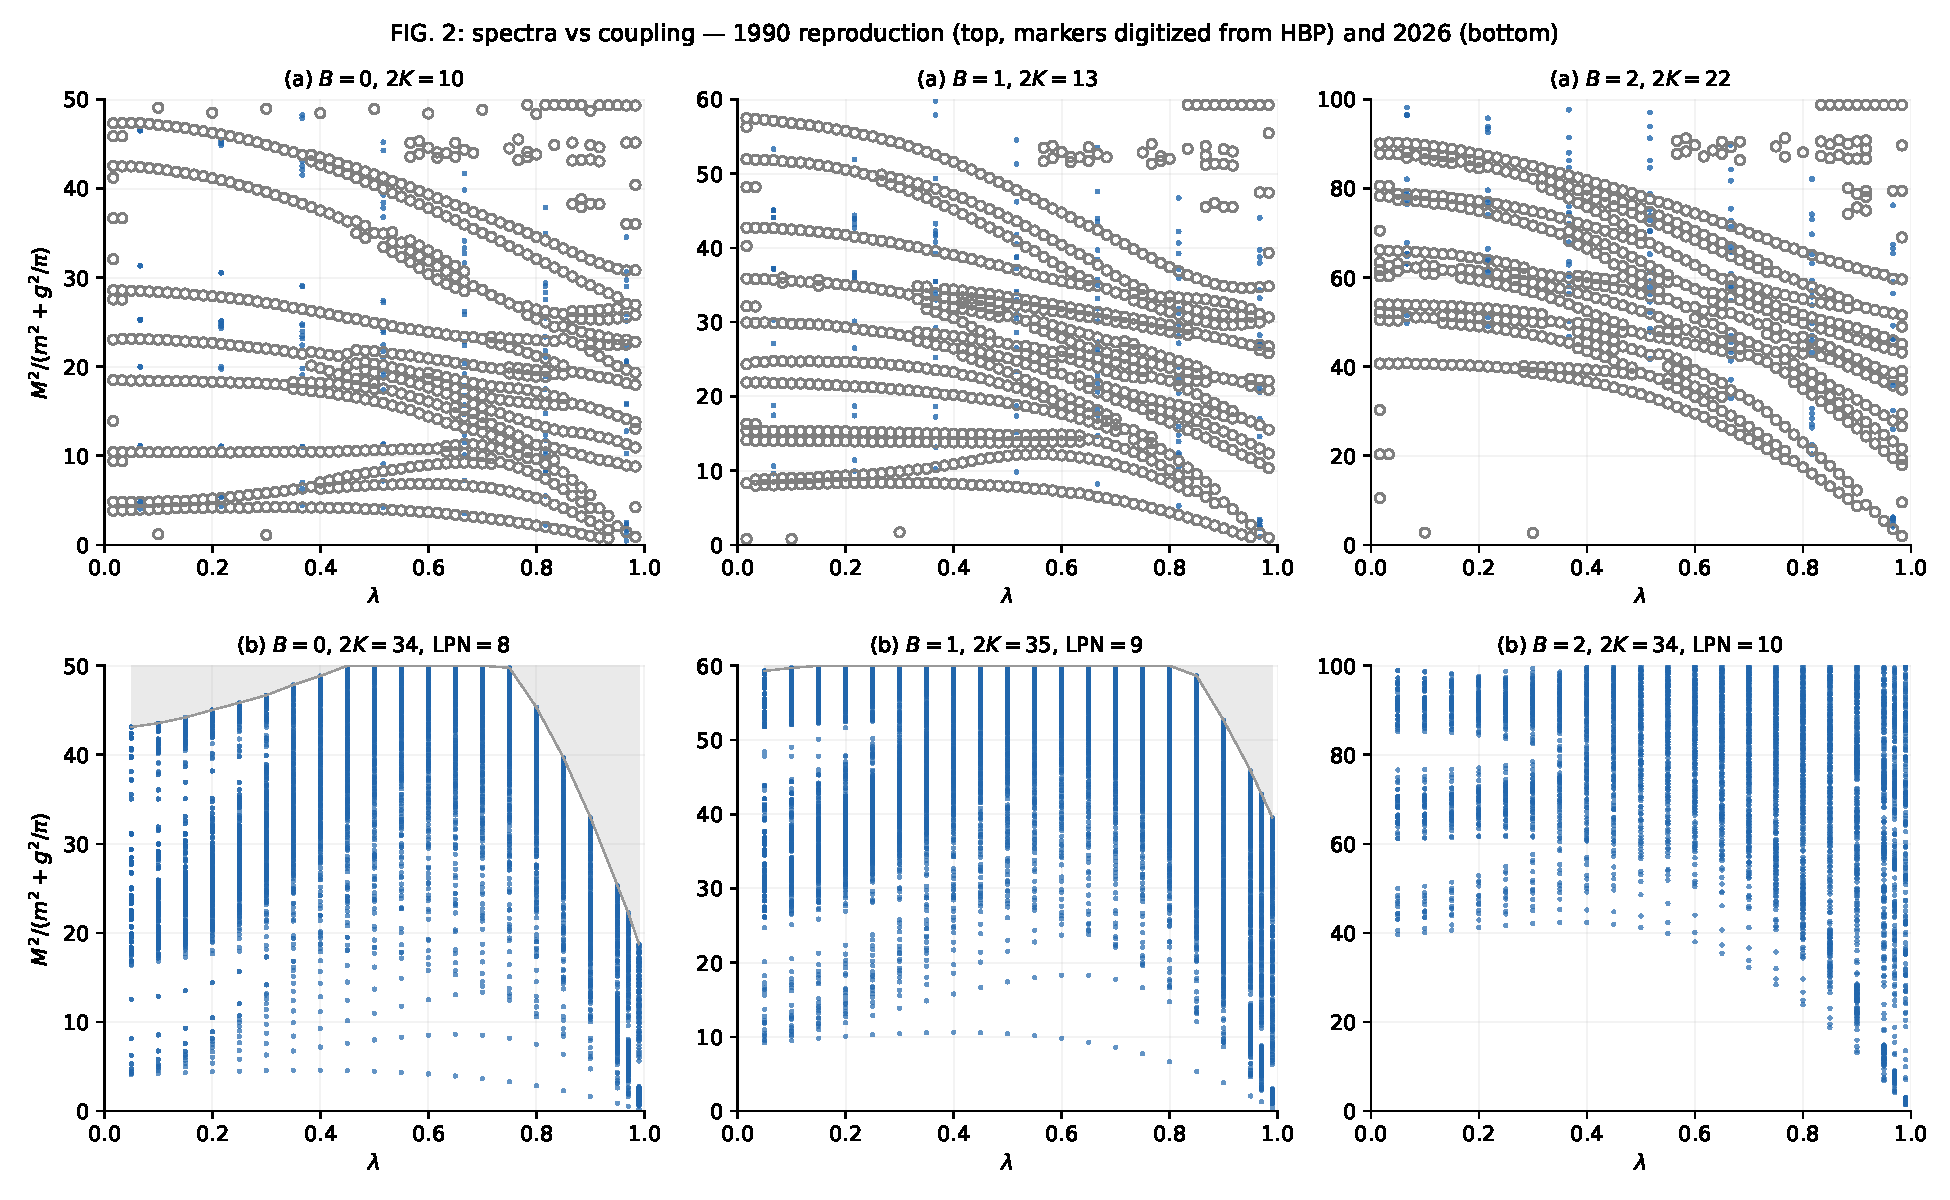
\includegraphics[width=\textwidth]{figs/fig2_spectra.pdf}
\caption{Spectra against the coupling $\lambda = [1+\pi m^2/g^2]^{-1/2}$,
$N=3$, all Hamiltonians standard, no fits.  Top: $B=0,1,2$ at
$2K = 10, 13, 22$, untruncated, markers digitized from Fig.~2 of
Ref.~\cite{Hornbostel:1988fb} (panel-to-$B$ assignment recovered; the
original caption omits it).  Bottom: $2K = 34, 35, 34$ at Fock truncation
$\mathrm{LPN} = 8, 9, 10$, lowest 250--400 states; the gray region marks
$M^2$ above the highest computed level, where states exist but are not
computed.}
\label{fig:spectra}
\end{figure*}

Figure~\ref{fig:spectra} is the coarsest and most complete comparison: the
full spectrum, scattering states included, across the coupling.  At the
1990 resolutions our levels sit inside the digitized markers across all
three baryon sectors.  At $2K = 34$ the same panels fill in: the level
density grows roughly linearly with $K$, isolated bound states remain
visible under the multi-hadron bands, and every level flows to zero at the
chiral point as Sec.~\ref{sec:massless} requires.  A resolution lesson
surfaced in drafting this panel and is worth recording.  At small
$\lambda$ a state of $L$ partons sits near $M^2/(m^2+g^2/\pi) \approx
L^2$, so matching the untruncated 1990 window requires Fock depth, not
resolution; a first attempt at $2K = 50$ with $\mathrm{LPN} = 6$ was
missing the entire upper half of the original panel, structurally.

\begin{figure}
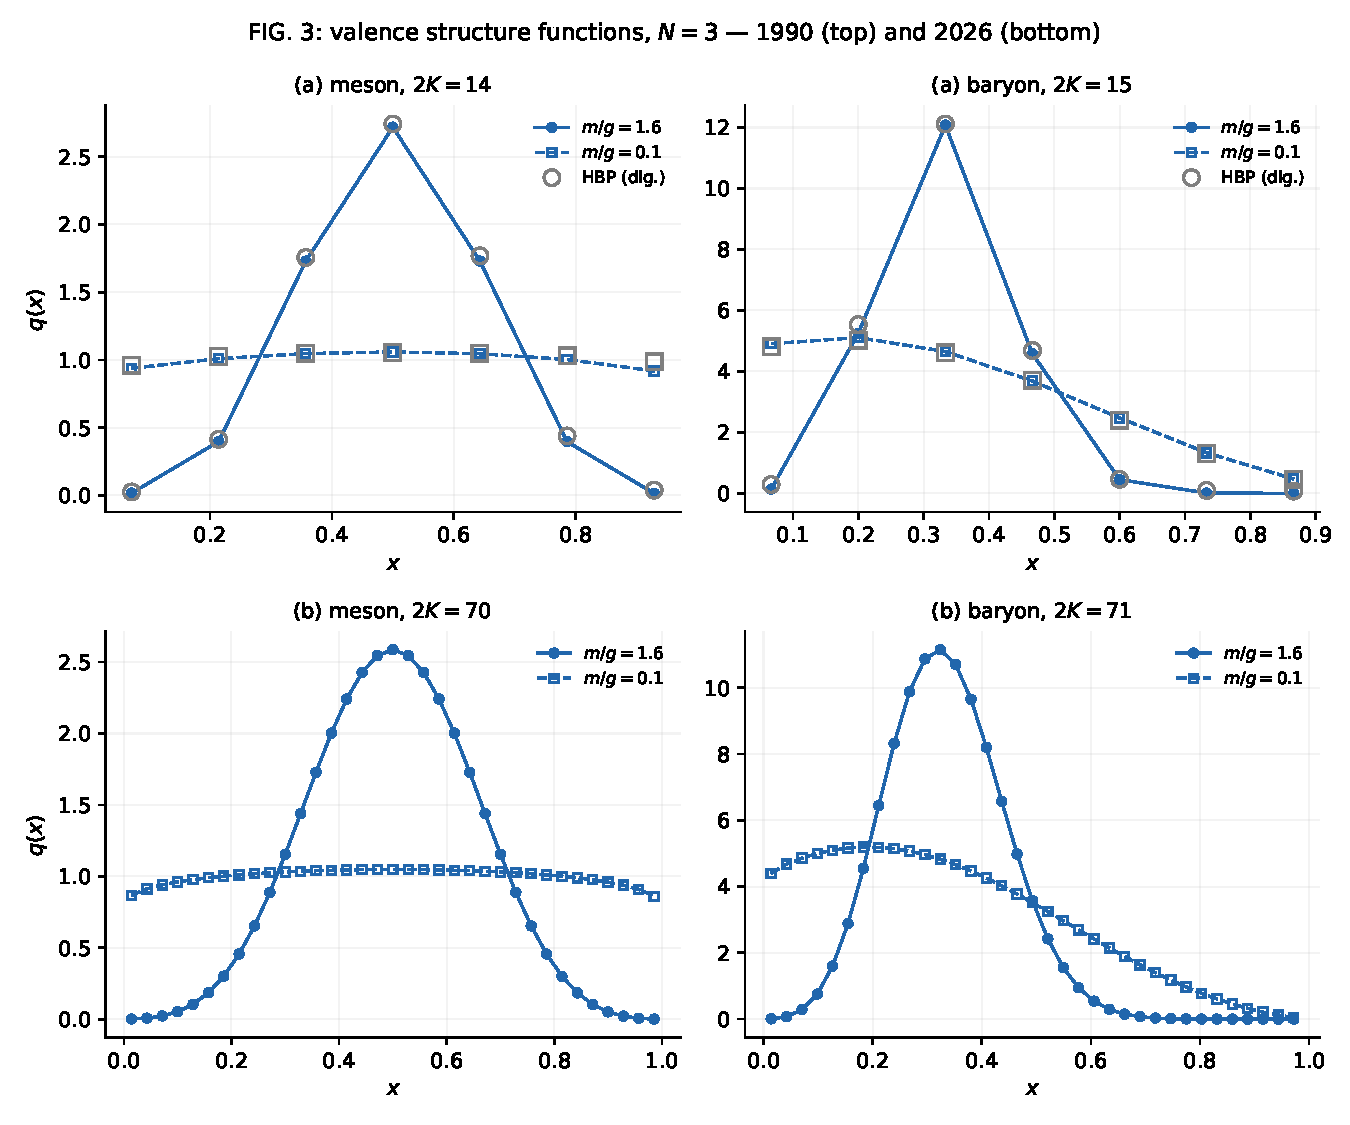
\includegraphics[width=\columnwidth]{figs/fig3_valence.pdf}
\caption{Valence structure functions, $N=3$, $m/g = 1.6$ (filled) and
$0.1$ (open), standard Hamiltonian, ground states, no fits.  Top:
$2K = 14$ (meson) and $15$ (baryon), the values recovered for the 1990
figure, whose caption omits them; markers digitized from Fig.~3 of
Ref.~\cite{Hornbostel:1988fb}.  Bottom: $2K = 70$ and $71$ at
$\mathrm{LPN} = 4$ and $5$.}
\label{fig:valence}
\end{figure}

The valence structure functions (Fig.~\ref{fig:valence}) repeat the
pattern.  At the recovered 1990 resolutions the digitized markers ring our
points; at $2K = 70$ the same curves are smooth.  The physics is as the
original described: weak coupling peaks the meson near $x = 1/2$ and the
baryon near $1/N$, and strong coupling flattens both toward the massless
distributions of Sec.~\ref{sec:massless}.

% \itodo{Fig. 4 (higher-Fock structure functions incl. qbar and the pion
% content of the baryon) needs its 2026 runs at both couplings — add to
% phase4a_config and draft the paragraph here.}

\begin{figure*}
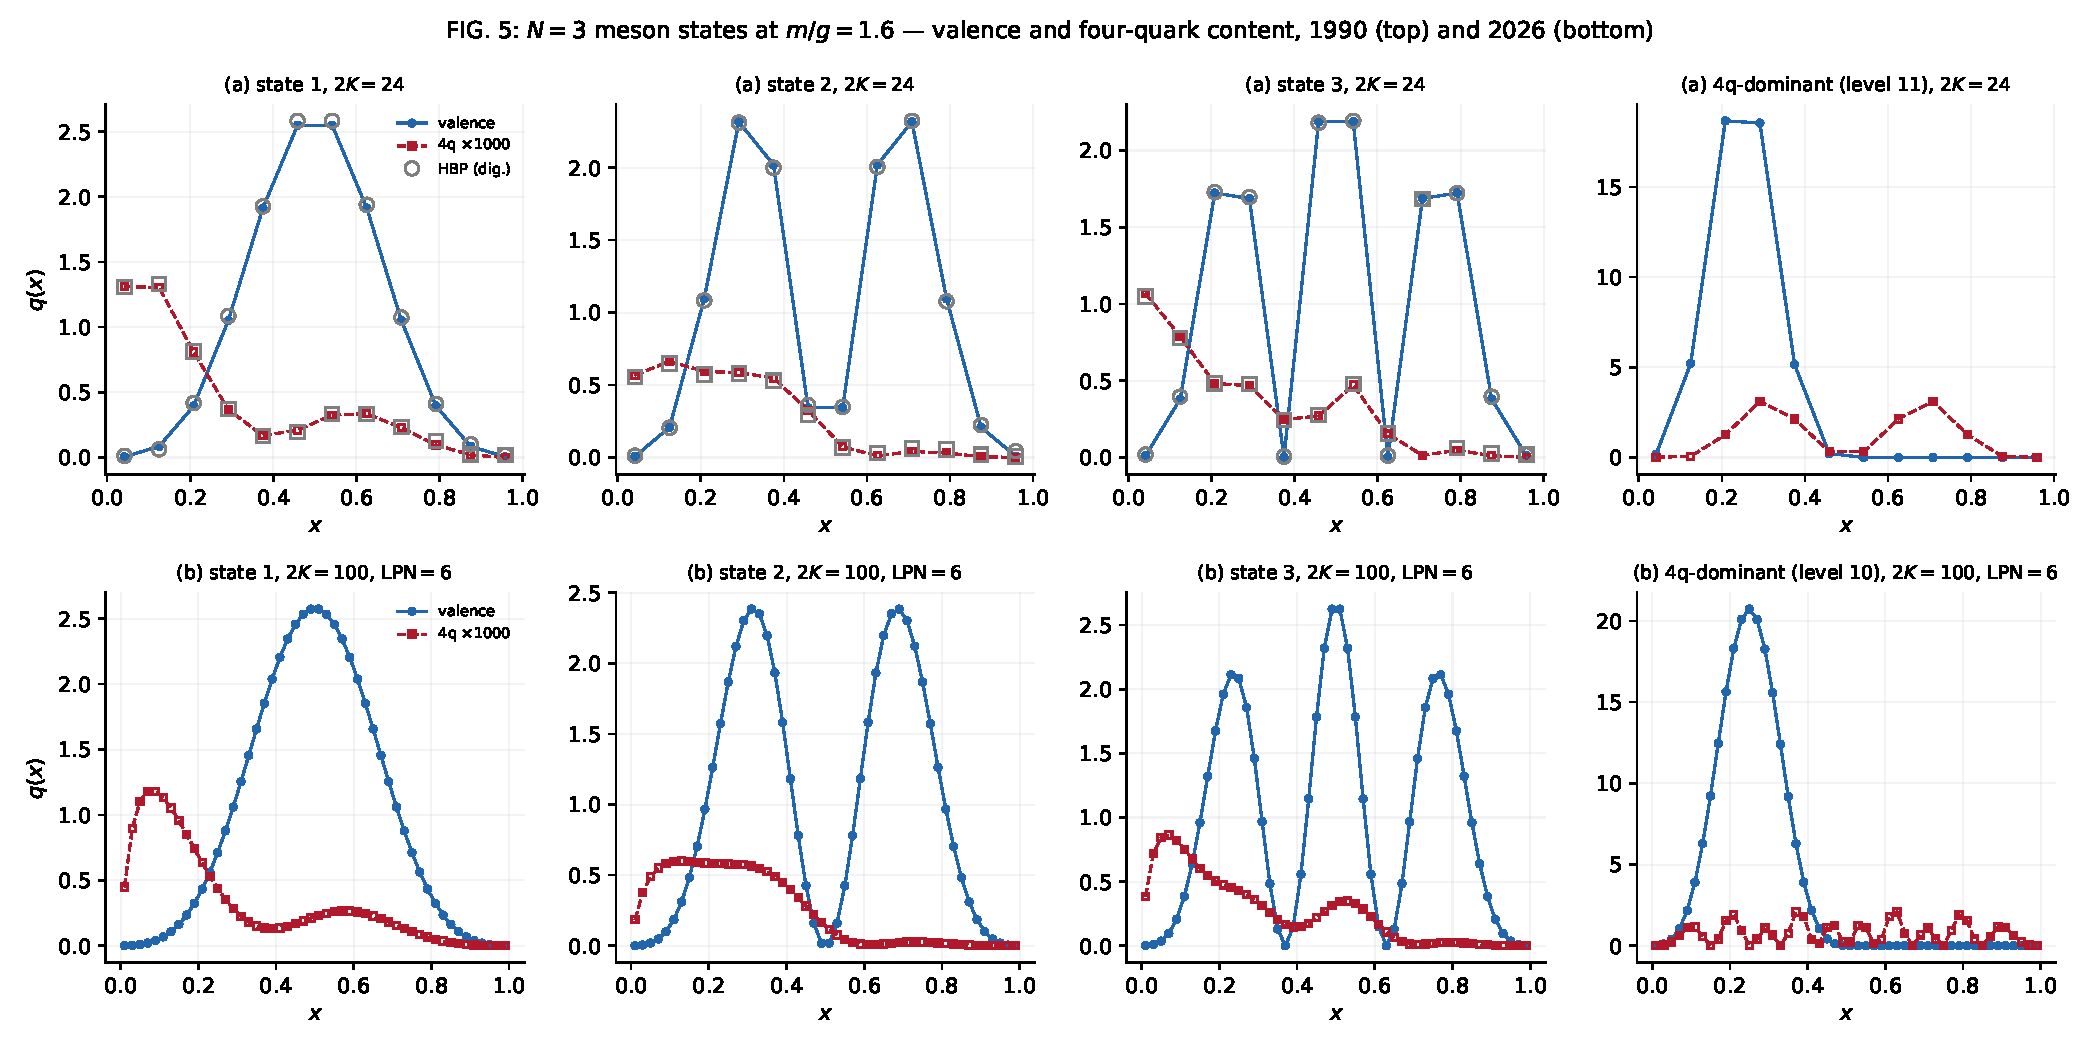
\includegraphics[width=\textwidth]{figs/fig5_meson_wf.pdf}
\caption{$N=3$ meson states at $m/g = 1.6$, standard Hamiltonian: valence
(solid) and four-quark (dashed, scaled by the stated multiplier) content.
Top: $2K = 24$, untruncated, markers digitized from Fig.~5 of
Ref.~\cite{Hornbostel:1988fb}; the last panel's digitized markers are
withheld because that panel of the original carries a second axis and the
traces calibrate to it.  Bottom: $2K = 60$, $\mathrm{LPN} = 6$, lowest 40
states.  The last column selects the first state whose four-quark Fock
weight exceeds one half, rather than a fixed level number.}
\label{fig:mesonwf}
\end{figure*}

The meson excitations (Fig.~\ref{fig:mesonwf}) add a selection question
the 1990 paper answered by inspection.  Its Fig.~5(d) showed ``the
eleventh state,'' identified in the text as two $q\bar q$ pairs in the
$\pi\pi$ continuum.  We select that physics directly: the last column
shows the first state whose four-quark Fock weight exceeds one half,
computed from the block-diagonal norm (Sec.~\ref{sec:exotics}).  At
$2K = 24$ the selector lands on level 11 --- the 1990 identification,
recovered independently.  At $2K = 60$ it lands on level 12, and the
four-quark profile peaks near $x = 1/4$: two pairs, each near half the
momentum, as the continuum interpretation requires.

\begin{figure*}
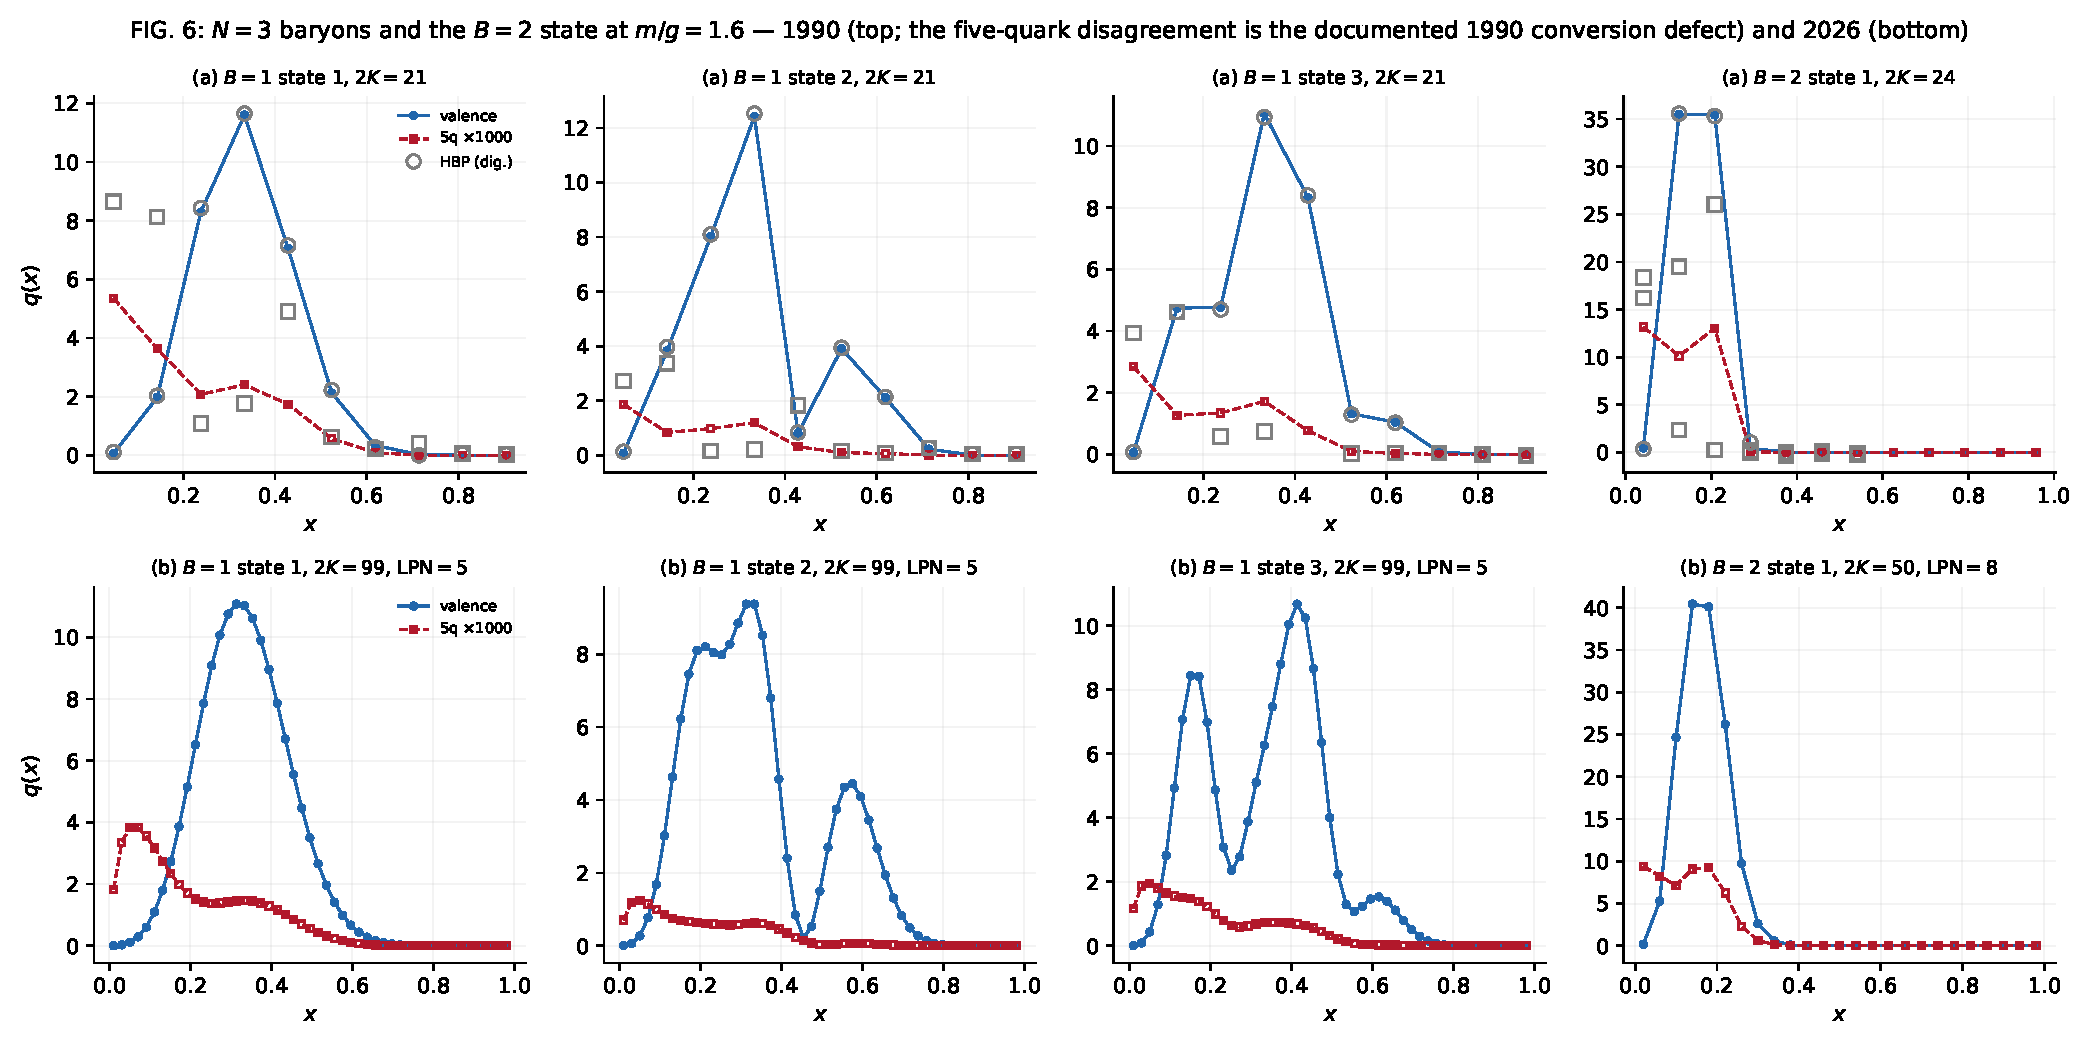
\includegraphics[width=\textwidth]{figs/fig6_baryon_wf.pdf}
\caption{$N=3$ baryon states and the $B=2$ state at $m/g = 1.6$, standard
Hamiltonian: valence (solid) and five- or eight-parton (dashed, scaled)
content.  Top: $2K = 21$ ($B=1$) and $24$ ($B=2$, a value the 1990
caption omits), untruncated, markers digitized from Fig.~6 of
Ref.~\cite{Hornbostel:1988fb}.  Bottom: $2K = 69$ and $50$ at
$\mathrm{LPN} = 5$ and $8$.  The five-quark disagreement in the first
three top panels is deliberate; see text.}
\label{fig:baryonwf}
\end{figure*}

Figure~\ref{fig:baryonwf} contains the one part of the 1990 paper we can
reproduce only by disagreeing with it.  The published five-quark curves of
its Figs.~6(a)--(c) sit 25--43\% from ours, while everything around them
agrees.  The evidence localizes the defect downstream of the 1990
eigensolve.  A preserved 1990 eigenvector reproduces the published valence
curves to one percent yet sits 43\% from the published five-quark curve,
which exonerates the color sums, the Hamiltonian, and the
diagonalization; what remains is the era's lost momentum-space conversion
program, which cannot be run.  Two checks support our curves.  The
five-quark coefficients satisfy the constraint the eigenproblem itself
imposes, $c_5 = -(H_{55} - \omega N_{55})^{-1} H_{53}\, c_3$, computed
from our matrices and the published valence.  And the $B=2$ panel, drawn
from the same machinery at the same coupling, agrees with the published
eight-parton curve to better than half a percent --- the control for
everything to its left.

\begin{figure}
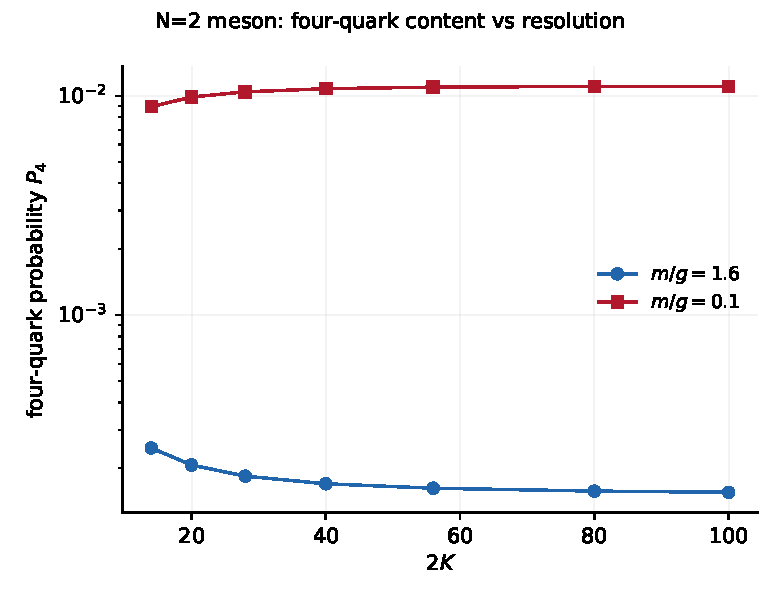
\includegraphics[width=0.8\columnwidth]{figs/fig22_p4_vs_K.pdf}
\caption{Four-quark probability $P_4$ of the $N=2$ meson ground state
against resolution, $m/g = 1.6$ and $0.1$, standard Hamiltonian,
$\mathrm{LPN} = 4$, no fits.  The published data reach $2K = 20$ (thesis
Fig.~22 of Ref.~\cite{Hornbostel:1988ne}); this extends the scan to
$2K = 100$.}
\label{fig:p4}
\end{figure}

One published measurement of this kind existed only in the thesis: the
$K$ dependence of higher-Fock content, at two resolutions.
Figure~\ref{fig:p4} extends it by a factor of five.  The two couplings
move in opposite directions.  At strong coupling the four-quark
probability grows with $K$ and saturates near one percent; at weak
coupling it falls toward a few parts in $10^4$.  Higher-Fock content is
not a fixed small number but a resolution-dependent one, and any
comparison of Fock truncations across $K$ inherits that dependence
(Appendix~\ref{app:budget}, the truncation component).

% 06-massless-limit — the analytic anchor; kept short on purpose
\section{Massless mesons and baryons in the $m/g \to 0$ limit}
\label{sec:massless}

At $m = 0$ the spectrum contains towers of exactly massless hadrons.  The
construction is Sec.~VI of Ref.~\cite{Hornbostel:1988fb} and survives
unchanged, so we record only what this paper uses.  The color currents
$V^a_k$ obey a Kac--Moody algebra, and the interacting part of $P^-$ is a
quadratic form in them.  States created purely by currents, and for baryon
number by a composite baryon operator, are annihilated by it.  Massless
mesons, baryons, and multi-hadron states therefore exist at every
resolution $K$, not merely in the limit.  The massless baryon's valence
distribution is closed-form,
\begin{equation}
  q(x) \;=\; N(N-1)\,(1-x)^{N-2},
  \label{eq:massless-sf}
\end{equation}
and collapses at $N = 2$ to the flat meson distribution.  For U($N$) the
extra U(1) current promotes these states to free bosons at
$M^2 = g^2/2\pi$: the Schwinger mechanism, and the sharpest statement of
how SU($N$) and U($N$) differ in two dimensions.

Three later results lean on this section.  The identically-zero last row of
Table~\ref{tab:tableone} is exact and $K$-independent; our solvers
reproduce it at every resolution as a structural check.  The chiral fits of
Sec.~\ref{sec:chiral} use masslessness as the fixed endpoint any
$M^2(m/g)$ form must respect.  And the exotics search of
Sec.~\ref{sec:exotics} inherits a boundary condition: multi-hadron states
are exactly massless at $m = 0$, so every binding energy we measure must
vanish in the chiral limit.  A candidate whose $\Delta$ fails to do so is
diagnosing its own systematics, not new physics.

% 07-error-budget
\section{Convergence and the error budget}
\label{sec:budget}
% TODO: draft after Phase 1 regeneration (post-450d724 numbers only)

% 08-chiral-region
\section{The chiral region}
\label{sec:chiral}
% TODO: draft against v1 freeze; mandatory caveats in plan
% Table I lives here: \label{tab:tableone} on the table environment.

% 09-exotics — the tetraquark/hexaquark search; no 1990 counterpart
\section{Tetraquark and hexaquark candidates}
\label{sec:exotics}

The 1990 paper met multiquark states twice without pursuing them: the
$\pi\pi$-continuum meson state of its Fig.~5(d) and the two-baryon state of
its Fig.~6(d).  This section pursues them.  Large-$N$ analyses of
meson--meson scattering predict a tetraquark pole very close to the lowest
two-meson threshold~\cite{Sazdjian:2025mqg,Sazdjian:2024vlm,Lucha:2017gqq,
Chen:2019dbk}, and tensor-network studies at finite density find
multibaryon bound states of striking robustness~\cite{Silvi:2016cas,
Silvi:2019wnf}.  Both claims are testable here at finite $N$, in the
original quantization, with controlled resolution systematics.

Three diagnostics run over every level of the $B=0$ and $B=2$ spectra.
The Fock-sector weight, computed exactly from the block-diagonal norm,
classifies each state by its dominant parton number; a tetraquark
candidate is a level whose four-parton weight exceeds one half, not a
level number chosen by eye.  The binding energy is a same-$K$ correlated
difference, $\Delta = M - 2M_{\rm thresh}$, with state and threshold on
one grid; the analysis code refuses any other construction, since
differencing two separate extrapolations double-counts every shared
systematic.  And the drift of $\Delta$ with resolution separates the two
hypotheses: a discretization artifact runs with the grid, a bound state
does not.  At $N=4$ the meson, baryon, and $B=2$ sectors share even
$K_{\rm code}$, so exact same-$K$ differences exist for every threshold;
at $N=3$ the baryon grid is odd, and the two-baryon study runs at $N=4$
for exactly that reason.

\begin{figure*}
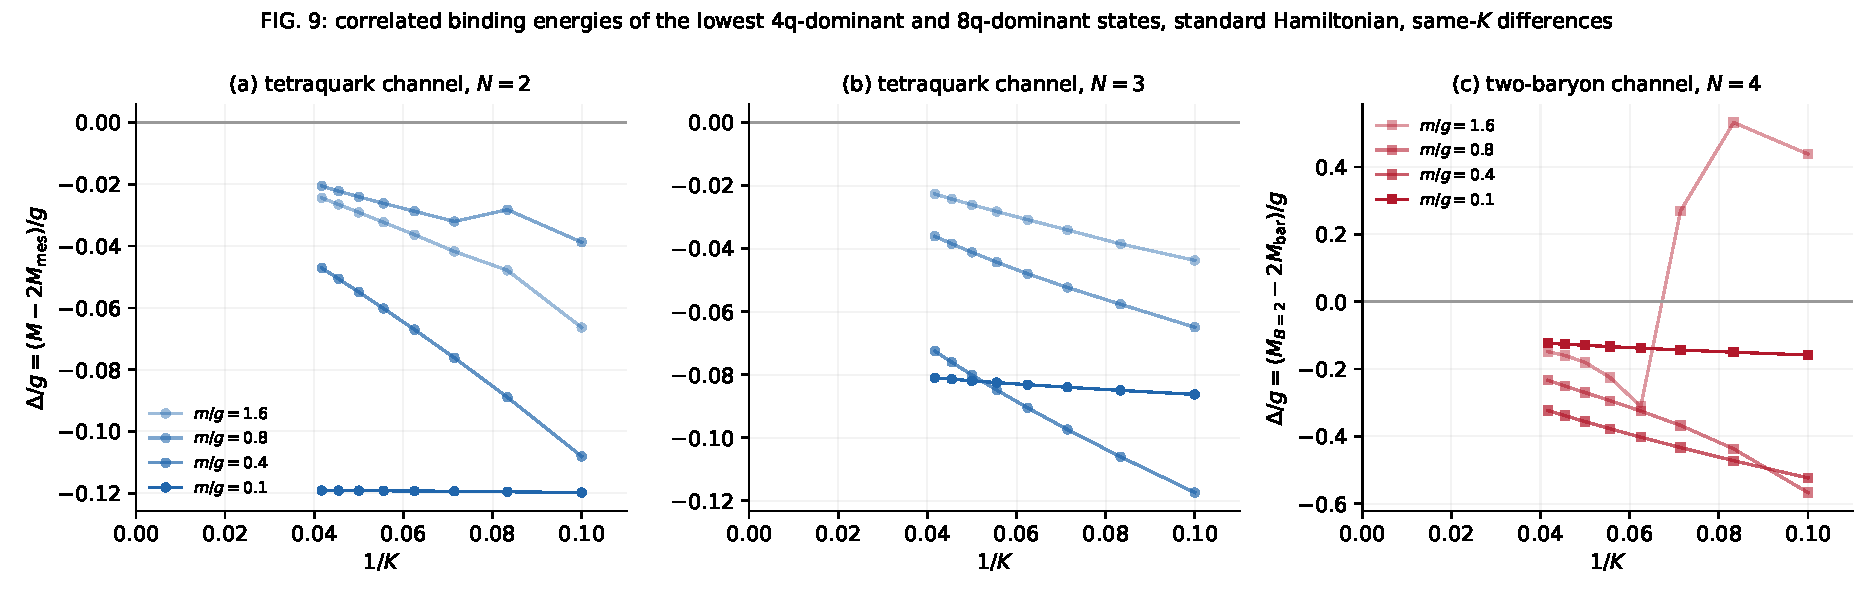
\includegraphics[width=\textwidth]{figs/fig9_exotics.pdf}
\caption{Correlated binding energies against $1/K$, standard Hamiltonian,
even $2K = 20$--$48$, Fock truncations $\mathrm{LPN} = 6$ ($B=0$, $N=2,3$)
and $10/6$ ($B=2/B=1$, $N=4$), $m/g$ as labeled, no fits drawn.  (a), (b):
lowest four-quark-dominant $B=0$ level minus twice the same-$K$ meson
mass.  (c): $B=2$ ground state minus twice the same-$K$ baryon mass.  The
$m/g=1.6$ discontinuity in (c) is a level crossing, discussed in the
text.}
\label{fig:exotics}
\end{figure*}

Figure~\ref{fig:exotics} shows both channels.  The pattern splits cleanly
by coupling.  At weak coupling the four-quark deficit drains away with
resolution: extrapolated in $1/K$, the $N=2$ channel gives
$\Delta/g = \numExoTetraNTwoMgOnepSix$ at $m/g = 1.6$, consistent with
zero.  The $N=3$ channel gives $\numExoTetraNThreeMgOnepSix$: a
threshold-hugging whisper, two to three spreads below zero, precisely the
regime where the large-$N$ scattering analyses place their near-threshold
pole.  We flag it as a candidate and decline to claim it; the quoted
spread is a fit-ensemble width, not a full budget.

Strong coupling is different in kind.  At $m/g = 0.1$ the lowest
four-quark-majority level sits below twice the meson mass by
$\numExoTetraNTwoMgZeropOne$ at $N=2$ and
$\numExoTetraNThreeMgZeropOne$ at $N=3$, and the deficit does not move:
it is flat in $1/K$ at the fourth decimal across a factor of 2.4 in
resolution.  By the drift criterion this is a converged sub-threshold
state.  What it is a state \emph{of} is less clean, and we state the
mixing plainly: its four-quark weight is 0.5--0.7, not 0.99, so it is a
strongly mixed object rather than a compact tetraquark, and at this
coupling the distinction between ``bound two-meson molecule'' and
``four-quark state'' may not survive scrutiny.  The massless limit
enforces $\Delta \to 0$ at $m/g \to 0$ (Sec.~\ref{sec:massless}), so the
binding must eventually release; mapping where sits beyond this first
survey.

The two-baryon channel echoes the tensor-network finding.  The $N=4$
$B=2$ ground state is structurally a hexaquark --- its eight-parton Fock
weight is \numHexaEightqWeight{} at $2K=48$, $m/g=0.1$ --- and it sits
below twice the baryon mass at every resolution reached, with
$\Delta/g = \numExoHexaMgZeropOne$ at $m/g = 0.1$ and
$\numExoHexaMgZeropFour$ at $0.4$.  At $m/g = 1.6$ the channel changes
character between $2K = 28$ and $32$: the correlated difference jumps
sign, the signature of a level crossing in one of the sectors, and we
exclude the pre-crossing points from the fit and quote
$\numExoHexaMgOnepSix$ with its accordingly useless spread.  Identifying
which levels cross, and whether the weak-coupling channel binds at all,
needs the crossing resolved rather than averaged over.

Two closing caveats bound this section's claims.  All of it is
standard-Hamiltonian physics at couplings above the validity boundary of
Sec.~\ref{sec:budget}, where that Hamiltonian is reliable; none of it
extrapolates into the chiral region.  And every binding energy here is a
statement about this theory's spectrum at finite $N$, not yet matched to
the unitarized large-$N$ amplitudes it was motivated by; that comparison
needs the scattering normalization those analyses use, and we leave it as
the natural next step.

% \itodo{NF=2 manifestly-exotic channels (Python-only capability) — the
% flavor-nonsinglet probe runs; a v2 candidate if time allows.}

% 10-modern-methods — the section HBP wrote as one paragraph and one figure.
% Subsection D ends the section completely: the equal-time cross-check, if it
% arrives, is added as its own file (10e) referenced from nowhere else.
\section{Comparison with modern methods}
\label{sec:modern}

The 1990 paper compared against the two external results then available:
't~Hooft's large-$N$ solution and Hamer's finite-lattice SU(2)
spectrum~\cite{Hamer:1982nc}.  The modern record is far richer, and this
section is organized by what each method can check.

\subsection{Large $N$ and integrability}
\label{sec:modern-largeN}

The 't~Hooft equation is now solved to essentially arbitrary precision: its
equivalence to a TQ-Baxter system~\cite{Ambrosino:2023dik,Litvinov:2024aa}
turns the large-$N$ meson spectrum into a benchmark exact for our purposes.
Our finite-$N$ masses, rescaled to 't~Hooft's normalization
(Appendix~\ref{app:units}), approach these values with the expected $1/N^2$
systematics, updating Fig.~8(b) of Ref.~\cite{Hornbostel:1988fb} with error
bars on both axes' inputs.  The same rescaled comparison exposes what
large $N$ misses at strong coupling --- light baryons, and the U(1)
distinction of Sec.~\ref{sec:massless} --- exactly as the original argued,
now with the residuals quantified.

\subsection{Lattice}
\label{sec:modern-lattice}

Hamer's SU(2) finite-lattice masses remain the only equal-time spectrum
across the full coupling range at $N = 2$.  We compare against his published
Table~1, whose stated uncertainties at weak coupling are of order the values
themselves; a digitization of his figure would suggest a precision his own
table disclaims, and we deliberately do not use one.  Within those bars,
agreement is complete, including the $N = 2$ identity $M_{\rm bar} = M_{\rm
mes}$ that his data was the first to exhibit.  Modern overlap-fermion
lattice work confirms the expected infrared behaviour at
$(N_c, N_f) = (2,1)$ and $(3,1)$~\cite{Karthik:2023vjv}, though without
spectrum tables to compare digit-for-digit.

\subsection{Tensor networks and quantum hardware}
\label{sec:modern-tn}

Hamiltonian-lattice calculations with matrix product states now reach
SU(2)~\cite{Silvi:2016cas,Banuls:2017ena} and
SU(3)~\cite{Silvi:2019wnf,Hayata:2023bgh} in one dimension, and variational
quantum hardware has produced SU(2) meson and baryon
masses~\cite{Atas:2021ext} with SU(3) preparations
following~\cite{Farrell:2022wyt}.  These are staggered-fermion,
finite-lattice-spacing computations, so the honest comparison is at matched
continuum extrapolations rather than raw numbers; where the published works
quote continuum values, we tabulate them beside ours.  Precision benchmarks
in the Schwinger model~\cite{Banuls:2013jaa,Dempsey:2022nys} calibrate what
tensor-network methods achieve at U(1), and our equal-time
exact-diagonalization cross-checks (Appendix~\ref{app:data}) reproduce them
in our own conventions.  No public code exists for any of the SU($N$)
tensor-network calculations above; the open pipeline released with this
paper is, to our knowledge, the first reproducible finite-$N$ spectrum code
in either quantization.

\subsection{The chiral-exponent tension}
\label{sec:modern-tension}

One discrepancy in this landscape is structural, and we state it as the open
question it is.  Every light-front determination of the finite-$N$ chiral
exponent --- this work, lightcone conformal truncation~\cite{Anand:2021qnd},
and $1/N$-corrected 't~Hooft perturbation theory~\cite{Kochergin:2024aa} ---
finds $M^2 \propto (m/g)^\alpha$ with $\alpha \to 1$, while the one
equal-time measurement, an MPS study of SU(2) over $m/g \in
[0.1, 0.4]$~\cite{Banuls:2017ena}, reports $\nu = 0.700(29)(11)$ for
$M \propto (m/g)^{\nu}$, i.e.\ $\alpha \simeq 1.4$: consistent with the
bosonization prediction and several standard deviations from the light-front
value.  The methods share no assumption more specific than quantization
itself --- but they differ in precisely the one all light-front schemes
share, the trivial vacuum, which is what an anomalous chiral exponent is
about.  The equal-time side of the ledger is not yet decisive either: the
measured window spans a factor of four in $m/g$, not a decade, and no
SU($N$) analogue of the additive staggered mass shift~\cite{Dempsey:2022nys}
--- the same order in the lattice spacing as the mass being fitted --- has
been published or applied.  Resolving the tension requires an equal-time
computation in the same chiral window with that renormalization under
control; it is beyond the published record, and beyond this paper.

% 11-prospects — what this machinery can reach next
\section{Prospects}
\label{sec:prospects}

Four extensions are within reach of the machinery described here, in rough
order of readiness.

\emph{QCD coupled to QED with physical charges.}  The colour-contraction
tables already compute both Fierz structures, and the U(1) exchange reuses
the $-1/N$ index structure with different weights, so
$H = H_{\rm QCD} + (e^2/g^2) H_{\rm QED}$ is available as a reweighting of
matrix elements already built, with one build serving every charge ratio.
The validation ladder is clean --- bit-identity at $e = 0$, the exact
Schwinger mass at the U(1) point, isospin restoration --- but Gauss' law on
a circle admits only neutral states without a zero-mode subtraction: the
neutron and $\pi^0$ come free, the proton does not.

\emph{The U($N$) switch.}  The same reweighting at $e^2/g^2 \to$ pure U(1)
limit exposes the SU($N$)/U($N$) split of Sec.~\ref{sec:massless}
numerically; the thesis~\cite{Hornbostel:thesis} plots the SU(2)--U(2)
comparison that the 1990 article never showed, and reproducing it would
close the last unreproduced published figure of this program.

\emph{Zero modes.}  Our antiperiodic quantization removes the $k^+ = 0$ mode
by fiat.  In two-dimensional models where zero modes have been included
dynamically, low-lying masses shift by as much as
$\sim 20\%$~\cite{Muller:1998mk}, so their absence is a genuine systematic
of unknown size for this paper's absolute masses --- though not the cause of
the weak-coupling failure, which a continuum solver with no zero-mode
truncation reproduces exactly (Sec.~\ref{sec:budget}).  Collective-variable
treatments that tensor a zero-mode sector onto the Fock basis exist and are
compatible with our solver architecture.

\emph{An equal-time computation in the same chiral window.}  The sharpest
open discrepancy this paper documents --- light-front methods finding
$M^2 \propto (m/g)^{\alpha}$ with $\alpha \to 1$ where the one equal-time
measurement suggests $\alpha \approx 1.4$ (Sec.~\ref{sec:modern}) --- will
not be settled by more $K$.  It needs an equal-time calculation with a
controlled additive mass renormalization at finite $N$, over a decade in
$m/g$ rather than a factor of four.  The missing theoretical ingredient is
the SU($N$) analogue of the staggered-fermion mass shift known for the
Schwinger model~\cite{Dempsey:2022nys}; deriving it is, in our view, the
single most valuable piece of new work available in this corner of field
theory, and the natural subject of a companion study.


\appendix
% app-a-budget
\section{Error-budget definitions}
\label{app:budget}
% TODO: component definitions + correlations after Phase 1

% app-b-do-not-retry — negative results, kept so they are not re-tried.
% Source: docs/weak-coupling-limit.md at blob b2a49a2 (pinned; gate G5).
\section{Approaches measured not to work}
\label{app:donotretry}

Every strategy below was implemented and measured against the
standard-Hamiltonian weak-coupling problem of Sec.~\ref{sec:budget}, then
rejected.  We record them because each is the obvious next idea.  Each also
fails invisibly from inside the fit, which is the property that makes the
underlying problem dangerous.  Numbers refer to the
Table~\ref{tab:tableone} channels at $m/g \le 0.2$ unless stated.

\begin{description}
\item[More resolution.]  The remainder falls only as $K^{-a}$ with
  $a \to 0$.  Halving the uncertainty bracket at $m/g = 0.1$ requires
  raising $K$ by a factor of order $10^{4.9}$; at our smallest couplings
  the factor exceeds any conceivable computation.  Resolution buys nothing
  below the validity boundary.  That is the point.
\item[A confluent fit basis.]  Replacing the near-degenerate
  $\{K^{-1}, K^{-(1+a)}\}$ pair by a confluent basis spans the same space.
  The extrapolated mass is identical to one part in $10^{14}$.
\item[Committing to a single series order.]  Fixing the number of terms
  hides the order dependence rather than removing it: the next admissible
  term still moves the extrapolate by several percent.  Held-out resolution
  and consistency with the known chiral behavior prefer opposite ends of
  the admissible range, which is what an undetermined model order looks
  like.  The budget spans the ladder instead.  Constrained
  fits~\cite{Lepage:2001ym} are the principled alternative and would need
  priors on coefficients the endpoint physics leaves unconstrained; we did
  not pursue them.
\item[A validity floor on the fit windows.]  Raising the smallest admitted
  resolution shrinks the quoted spread severalfold while walking the
  central value monotonically, by many times the shrunken bar.  Variance is
  traded for bias, silently.
\item[Fitting the endpoint exponent freely.]  $M_0 - C\,K^{-p}$ is
  unidentifiable when the true $p$ is small.  $K^{-p}$ is nearly constant,
  $M_0$ and $C$ degenerate, and the fit lands an order of magnitude off
  with a residual of $10^{-7}$.  A perfect fit to the wrong answer.
\item[Summing the tail analytically.]  A Hurwitz-$\zeta$ resummation of the
  increment series validates at strong coupling.  It diverges where it is
  needed.
\item[Adding an explicit $K^{-a}$ column.]  With $a$ fixed from
  Eq.~\eqref{eq:endpoint-exponent}, the extrapolated masses land several
  times above the published values, and the fitted chiral exponent stays
  pinned to the grid artifact.  Inside a joint $(m/g, K)$ fit the same
  column produces variant spreads of hundreds of percent and negative
  masses.
\end{description}

The common failure mode deserves the emphasis: every rejected strategy
improved some internal diagnostic while degrading the answer.  Residuals,
held-out predictions, and spread statistics all reward flexibility inside
the reachable window, and the reachable window does not contain the physics
(Sec.~\ref{sec:budget}).  Where we quote weak-coupling numbers from the
standard Hamiltonian, the bar carries the endpoint systematic in full.
Where we need the chiral region, we change the Hamiltonian, not the fit.

% app-c-units — conventions, and the two traps that cost us real time
\section{Units and conventions}
\label{app:units}

Masses are quoted as $M/g$ unless stated otherwise; $m/g$ is the quark mass in
units of the coupling.  The natural combination in this paper's normalization
is $g^2 N/2\pi$, whereas 't~Hooft's classic solution uses $g^2 N/\pi$; the
large-$N$ comparison in Sec.~\ref{sec:modern} therefore plots
$(2\pi/N)^{1/2}\,M/g$ against $(2\pi/N)^{1/2}\,m/g$, exactly as Fig.~8(b) of
Ref.~\cite{Hornbostel:1988fb} did.  Spectra shown as functions of the coupling
use the compactified variable $\lambda = [1 + \pi m^2/g^2]^{-1/2}$, which maps
the free limit to $\lambda \to 0$ and the chiral limit to $\lambda = 1$, and
the dimensionless mass $M^2/(m^2 + g^2/\pi)$, both directly comparable to the
1990 figures.  In code units the resolution is $2K$ (integer, matching the
parity of the parton number) and single-parton momenta are odd integers
$k = 1, 3, \ldots$, so a structure function lives on $x = k/2K$ with measure
$dx = 1/K$.

Two conventions of Ref.~\cite{Hornbostel:1988fb} are traps for anyone
comparing against it, and we state them explicitly since both bit us.
First, \emph{the numbers printed in its Table~I are $M^2/(m^2+g^2/\pi)$,
although the column headers read $M/g$}.  The two agree at no coupling; the
identification was established by recomputing both quantities at the 1990
parameters and matching digit patterns, and our transcription of the table
carries the correction with full provenance.  Every comparison in this paper
converts to genuine $M/g$, and the cross-check that our conversion is right
--- recomputing the comparison in the table's native $M^2$ units --- is part
of the build (Appendix~\ref{app:data}).  Second, the parenthesized digits in
that table are \emph{not} error bars: they record the magnitude of the last
term retained in the extrapolation series, a convergence diagnostic the
authors themselves trusted only for $m/g \gtrsim 0.2$.  Where this paper
quotes an uncertainty, it is the full budget of Sec.~\ref{sec:budget}; where
it quotes the 1990 numbers, the parenthesis keeps its original meaning.

Captions in this paper state $N$, $B$, $2K$ (or the fit window), $m/g$, the
Fock-space truncation, and the Hamiltonian, for every panel; where the
original figure left a parameter unstated, the value we recovered and the
evidence for it are cited inline.

% app-d-data — reproducibility statement
\section{Data and code availability}
\label{app:data}

Both solvers --- the preserved 1988-era Fortran, unmodified, and the Python
port --- are public, together with every analysis script, the digitized
markers of all 1990 figure panels with their axis-calibration provenance,
and the per-figure data files, each carrying in its header the exact command
that regenerates it.  Every number quoted in this paper's prose is a macro
generated from those data files by a single extractor, with the repository
revision and input hashes recorded alongside; every figure is built by a
single driver that reads cached solver output and refuses to solve, so that
a missing input surfaces as an explicit run command rather than a silent
recomputation.  The equal-time exact-diagonalization used for the
Schwinger-model cross-checks of Sec.~\ref{sec:modern} is included.
% Repository URL + archived version DOI at v2 freeze.


\bibliography{refs}

\end{document}
